\chapter{Black Holes, White Holes, and Penrose Diagrams}

These notes follow Leonard Susskind's fourth lecture in the supplementary \emph{Topics in String Theory} track of \emph{Cosmology And Black Holes}, with curation by LazyingArt LLC. The lecture unfolds in two long arcs. In the first, Susskind returns to the near-horizon Schwarzschild geometry, asks how that local picture connects to the far region, and then uses observers, light rays, and the singularity to build the causal story of a black hole. In the second, after a short reset about proper distance, he introduces Penrose diagrams and uses them to separate the eternal Schwarzschild solution from the geometry of a black hole formed by collapse.

\section{Near-Horizon Recap and Choice of Variables}

Susskind opens by saying, in effect, let us go back to something familiar. Near the horizon the Schwarzschild geometry is approximately just flat spacetime, but only after one uses the right variables. The first is \(\rho\), the proper distance from the horizon; the second is \(\omega\), a dimensionless time variable built from the Schwarzschild time \(t\).

\begin{remark}
Throughout these notes the lecture's spoken \(m,g\) are standardized to \(M,G\), \(c=1\) is understood, and the metric signs are written in a consistent Lorentzian convention. When the spoken transcript slips verbally, the displayed equations below follow the mathematically intended form.
\end{remark}

The board recap is one of the clearest pieces of visual evidence in the lecture.

\begin{figure}[h]
\centering

\includegraphics[width=0.58\textwidth]{lecture_04_figure_02.png}
\end{figure}

The two equations written explicitly on the board are
\begin{align}
\omega &= \frac{t}{4MG},\\
ds^2 &= -\rho^2\,d\omega^2 + d\rho^2.
\end{align}
Susskind also reminds the audience of the defining geometric fact
\begin{equation}
\rho=0 \qquad \text{at} \qquad r=2MG.
\end{equation}
He does not re-derive the function \(\rho(r)\), and for this lecture he does not need to. What matters is only that \(r\) is not the proper distance from the horizon, whereas \(\rho\) is.

The metric above is then compared to the metric of the Euclidean plane in polar coordinates,
\begin{equation}
ds^2=\rho^2\,d\theta^2+d\rho^2.
\end{equation}
The comparison is the point. Near the horizon, the radial-time part of Schwarzschild is flat spacetime written in a hyperbolic-polar form, and \(\omega\) plays the role that \(\theta\) plays in ordinary polar coordinates. The only visible difference is the minus sign attached to the Lorentzian time direction.

This is not yet the whole black hole. It is the recalled local geometry near \(r=2MG\). But it immediately organizes the first picture: \(\omega\) runs from the remote past to the remote future, the lines of constant \(\rho\) are hyperbolae, and the horizon itself lies at \(\rho=0\). With that local picture back on the board, Susskind can ask the first genuinely new question of the lecture: what happens far from the black hole, and what sort of geometry interpolates between the two regimes?

\section{From the Horizon to Infinity: Why a Cigar Appears}

With the near-horizon metric re-established, Susskind turns to the opposite limit. Very far from the black hole, one should again recover flat spacetime. The issue is not whether the geometry becomes flat, but how the coefficient of the time term changes between the horizon and infinity.

Suppressing the angular part, the relevant radial-time sector of the Schwarzschild geometry is
\begin{equation}
ds^2=-\left(1-\frac{2MG}{r}\right)dt^2+\frac{dr^2}{1-\frac{2MG}{r}}.
\end{equation}
The transcript is verbally messy at this point, but the intended algebra is straightforward.

\paragraph{Asymptotic reduction.}
\begin{enumerate}
\item Take \(r\gg 2MG\), so that \(1-2MG/r\to 1\).
\item In that region the Schwarzschild coordinate \(r\) and the proper distance \(\rho\) are approximately the same:
\[
r\approx \rho.
\]
\item The metric therefore reduces to
\begin{equation}
ds^2\approx -dt^2+dr^2\approx -dt^2+d\rho^2.
\end{equation}
\item Using \(t=4MG\,\omega\), one has
\begin{equation}
dt^2=16M^2G^2\,d\omega^2.
\end{equation}
\item Hence far from the black hole,
\begin{equation}
ds^2\approx -16M^2G^2\,d\omega^2+d\rho^2.
\end{equation}
\end{enumerate}

This is the comparison that drives the rest of the section:
\begin{align}
ds^2 &\approx -\rho^2\,d\omega^2+d\rho^2
\qquad \text{near the horizon},\\
ds^2 &\approx -16M^2G^2\,d\omega^2+d\rho^2
\qquad \text{far away}.
\end{align}
The radial piece is not the interesting part. The interesting part is that the coefficient of \(d\omega^2\) changes from \(\rho^2\) near the horizon to a constant far away.

This also sharpens Susskind's remarks about clocks. Along a hovering worldline with \(d\rho=0\), the near-horizon metric gives
\begin{equation}
d\tau^2=\rho^2\,d\omega^2,
\end{equation}
so very close to the horizon only a very small proper time elapses for a given increment of \(\omega\). Far away, by contrast,
\begin{equation}
d\tau^2=16M^2G^2\,d\omega^2,
\end{equation}
so the same \(\omega\)-interval corresponds to the ordinary asymptotic time scale \(dt=4MG\,d\omega\).

At this point Susskind deliberately changes register. His own comment is that it is much easier to understand space than spacetime, so he introduces an ordinary Euclidean model with the same radial dependence in the angular coefficient:
\begin{equation}
ds^2\sim \rho^2\,d\theta^2+d\rho^2
\qquad \text{near the tip},
\end{equation}
and
\begin{equation}
ds^2\sim 16M^2G^2\,d\theta^2+d\rho^2
\qquad \text{far away}.
\end{equation}
This auxiliary geometry is not the black-hole spacetime itself. It is a visual aid for the changing coefficient.

The answer is the ``cigar'' geometry. Near the tip, the surface looks flat, just like ordinary polar coordinates near the origin. Far away, the distance around the \(\theta\)-direction no longer grows with \(\rho\); it approaches a constant circumference. Since \(\theta\) runs from \(0\) to \(2\pi\), that asymptotic circumference is
\begin{equation}
\oint ds=\int_0^{2\pi}4MG\,d\theta=8\pi MG.
\end{equation}
The geometric lesson is immediate. A large black hole corresponds to a cigar with a large asymptotic girth and therefore a blunter, less curved tip. A small black hole corresponds to a tighter cigar and larger curvature near the tip. Susskind does not introduce a curvature scalar here; the point is the picture.

He then returns to the main statement. The black-hole geometry is the one for which the coefficient of \(d\omega^2\) behaves like \(\rho^2\) near the horizon and like \(16M^2G^2\) far away. The cigar is the clearest ordinary-space analogue of that interpolation.

\section{Horizon Geometry and the Causal Sketch}

Once the interpolation has been made visual, Susskind returns to the Lorentzian spacetime picture. Here the lecture changes emphasis: from metric coefficients to causal meaning. The relevant board sketch is developed rather than pristine, but that is part of its value, since it preserves the way the argument accumulated on the blackboard.

\begin{figure}[h]
\centering

\includegraphics[width=0.60\textwidth]{lecture_04_figure_04.png}
\end{figure}

A cleaned version of the same structure is shown below. It is not meant as a literal transcription of every chalk stroke. It isolates the features that the transcript makes secure: crossed null lines, the central bifurcation point, fixed-\(\rho\) worldlines outside the horizon, and the wavy future and past boundaries that will later be identified as singularities.

\begin{figure}[h]
\centering
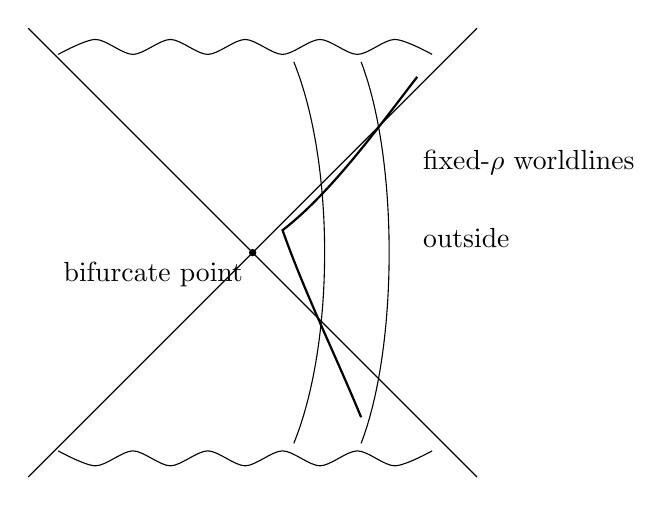
\begin{tikzpicture}[scale=0.95]
\draw (-3,-3) -- (3,3);
\draw (-3,3) -- (3,-3);

\draw plot[smooth] coordinates {(-2.6,2.65) (-2.1,2.85) (-1.6,2.65) (-1.1,2.85) (-0.6,2.65) (-0.1,2.85) (0.4,2.65) (0.9,2.85) (1.4,2.65) (1.9,2.85) (2.4,2.65)};
\draw plot[smooth] coordinates {(-2.6,-2.65) (-2.1,-2.85) (-1.6,-2.65) (-1.1,-2.85) (-0.6,-2.65) (-0.1,-2.85) (0.4,-2.65) (0.9,-2.85) (1.4,-2.65) (1.9,-2.85) (2.4,-2.65)};

\draw (0.55,-2.55) .. controls (1.10,-1.20) and (1.10,1.20) .. (0.55,2.55);
\draw (1.45,-2.55) .. controls (1.95,-1.25) and (1.95,1.25) .. (1.45,2.55);

\draw[thick] (2.20,2.35) .. controls (1.70,1.70) and (1.05,0.80) .. (0.40,0.30)
            .. controls (0.70,-0.55) and (1.10,-1.35) .. (1.45,-2.20);

\fill (0,0) circle (1.4pt);

\node[below left] at (0,0) {bifurcate point};
\node[right] at (2.15,1.20) {fixed-\(\rho\) worldlines};
\node[right] at (2.15,0.20) {outside};
\end{tikzpicture}
\end{figure}

The rule for reading all such sketches is one that Susskind repeats several times during the lecture.

\begin{definition}
In the reduced radial spacetime diagrams used here, radial light rays are drawn at \(45^\circ\).
\end{definition}

With that rule in hand, Susskind distinguishes two notions of horizon. The first is the \emph{bifurcate horizon}, which in his terminology is the central crossing point of the two null lines. The second, and physically more important one, is the \emph{event horizon}: the entire null surface that acts as the boundary of communication. Once this distinction is made, the sketch is no longer just a diagram. It becomes a statement about signaling. Light rays can fall inward through the horizon, but outward-directed radial light rays emitted from the interior do not escape to the exterior.

This is also where the fixed-\(\rho\) curves become physical. They represent observers hovering outside the black hole at constant proper distance from the horizon. In the lecture these worldlines are not yet Bob's story in full; they are first the geometric realization of what it means to remain outside the hole.

\section{Bob, Alice, Redshift, and the One-Way Barrier}

At this point the lecture becomes operational. Susskind moves from geometry to what particular observers can see, measure, and signal. Bob remains outside on a fixed-\(\rho\) worldline. Alice falls inward. The diagram is now read not merely as geometry but as an account of communication.

For Bob, the time parameter \(\omega\) is just the Schwarzschild time in units of \(4MG\):
\begin{equation}
t=4MG\,\omega.
\end{equation}
Thus the marks \(\omega=0,1,2,\dots\) along Bob's worldline are simply \(t=0,4MG,8MG,\dots\). He stays outside; he does not cross the horizon; he can keep reading off more and more time on his wristwatch.

Susskind first phrases the issue in terms of a photon, then quickly turns it into the more useful story of Alice, because Bob can only \emph{see} Alice by receiving light emitted from her. The causal sequence is then the following. Bob looks back and receives light from progressively later points of Alice's infalling worldline, but each received signal comes from a point still outside the horizon. He keeps seeing her wave. He keeps waiting. He keeps receiving signals. Yet the signals arrive farther and farther apart in his own proper time.

The crucial observation is that Bob never sees Alice cross the horizon. In the classical picture she appears to slow down, freeze just outside the horizon, and remain there. Susskind immediately refines that frozen picture into a statement about frequency. Alice is visible only because charges in her body are oscillating and emitting electromagnetic radiation. If Bob sees those oscillations slow down, then the light he receives must be redshifted. The lecture follows that redshift concretely:
\begin{itemize}
\item first optical light,
\item then infrared,
\item then long-wavelength radio,
\item and finally wavelengths so long that Bob effectively sees nothing at all.
\end{itemize}
The practical content of ``freezing at the horizon'' is therefore not that Alice remains optically visible forever, but that she fades away.

Susskind then asks for the reverse point of view. What does Alice see? Here the lecture is careful, because one can easily overread Bob's story and imagine that something dramatic must happen exactly at the horizon. Alice's experience says otherwise. She continues to see Bob even after she has crossed the horizon. Bob can still send signals inward to her. She, however, cannot send signals back out once she is inside. The horizon is therefore a one-way barrier, but not in the naive sense that each observer sees the same thing reversed. Bob sees Alice redshift and disappear; Alice sees Bob recede and redshift, but she does not see him vanish at her moment of crossing.

The lecture then sharpens the point with the feet-first thought experiment. Alice falls feet first, so the worldline of her feet crosses the horizon before the worldline of her head. If she simply continues to fall, nothing special happens at the horizon. She can still look back and see light coming from her feet, just as from any nearby object: not from the simultaneous event on the foot worldline, but from a slightly earlier point on it. In that sense there is no paradox. Horizon crossing by itself does not locally rip the body apart.

The trouble begins only if Alice changes her mind. Suppose her feet have crossed the horizon but her head tries to remain outside. Then her head must accelerate away from the black hole. The part already inside cannot accelerate enough to keep up, and in Susskind's description the body is stretched farther and farther until it breaks. This is not a generic statement that the horizon is locally singular. It is a more specific one: once part of an extended body has crossed the one-way barrier, trying to keep the rest of the body out requires an impossible kinematic arrangement.

\section{The Singularity, Coordinate Interchange, and White Holes}

Only after the horizon story has been made vivid does Susskind return to the Schwarzschild metric and asks where the singularity lies on the diagram. The order matters. He first separates the horizon from the singularity, and only then turns to the singularity itself.

The radial-time Schwarzschild sector is again
\begin{equation}
ds^2=-\left(1-\frac{2MG}{r}\right)dt^2+\frac{dr^2}{1-\frac{2MG}{r}}.
\end{equation}
The immediate fact is the sign change:
\begin{equation}
1-\frac{2MG}{r}>0 \quad \text{for} \quad r>2MG,
\qquad
1-\frac{2MG}{r}<0 \quad \text{for} \quad r<2MG.
\end{equation}
Outside the horizon the coefficient of \(dt^2\) is negative and the coefficient of \(dr^2\) is positive, so \(t\) is timelike and \(r\) spacelike. Inside the horizon the signs reverse. Susskind's point is that this does \emph{not} mean that the horizon is physically singular. It means that Schwarzschild coordinates become peculiar there: the coordinate roles interchange.

The lecture then gives this coordinate fact a geometric reading. One may imagine moving inward along a line of constant Schwarzschild time until one reaches \(r=2MG\). What happens next is not that one arrives at a special material surface. Rather, in these coordinates the \(r\)-lines turn and continue in a timelike direction. The important destination is not \(r=2MG\), but
\begin{equation}
r=0.
\end{equation}
That is the singularity. There tidal forces diverge, curvature becomes infinite, and, in Susskind's phrasing, all hell breaks loose.

The lecture insists on a further conceptual correction. At first one is tempted to think of the singularity as a \emph{place}. But on the causal sketch it is not drawn as a vertical worldline. It is drawn as a spacelike hyperbola-like boundary in the future. In Susskind's own language, it is more like a \emph{time} than a place: once one has crossed the horizon, the singularity lies ahead in one's future. This is why the black-hole interior is not merely a region from which one cannot communicate outward. It is a region in which every future-directed timelike or null path ends at the singularity.

From here the lecture takes its next conceptual jump. Schwarzschild is time-independent, and \(dt^2\) is unchanged under \(t\to -t\). The geometry is therefore time-reversal invariant. If a history in which Alice falls through a future horizon into a future singularity is allowed, then the time-reversed history must also solve the equations. That reversed history contains a past singularity and a past horizon from which matter may emerge. This is the \emph{white hole}: the time reverse of the black hole.

Susskind is quite explicit about the contrast between mathematics and plausibility. Mathematically, if Alice can pass in through a future horizon, then in the reversed solution she can pass out through a past horizon. Physically, however, that story looks absurd: Bob would see Alice suddenly ejected from a singular past. The lecture does not yet resolve that absurdity; it merely puts it on the table.

\section{Entropy and Why the White-Hole Half Is Unphysical}

The next section of the lecture is not a new geometric construction. It is a sustained explanation of why the time-reversed half of the eternal Schwarzschild solution is mathematically present but physically fantastical. Susskind does not treat this as a contradiction in the equations. He treats it as an entropy problem.

The structure of the argument is the familiar structure of irreversible physics. A bomb explodes and scatters debris; the time reverse, in which debris flies inward and delicately reassembles the bomb, is not forbidden by Newton's equations, but it is overwhelmingly improbable. A ball rolls down a hill; the reverse trajectory, in which it comes to rest exactly on the top, is possible but exquisitely unstable. Fifteen billiard balls scatter from a triangular rack; their spontaneous reconvergence into a perfect triangle is possible in principle and ridiculous in practice. An ice cube melts in a pot of hot water; the reverse process, in which an ice cube assembles itself from thermal motion, is again allowed by the microscopic equations and fantastically unlikely.

Susskind's point is that the white hole belongs in exactly this class. It is not \emph{impossible} in the formal time-reversal sense. It is the analogue of the entropy-lowering reverse trajectory. What Bob would see in the white-hole picture is not a forbidden process, but an outrageously special one: the black hole suddenly ejecting a full-fledged Alice. The lecture's language varies between ``nonsense,'' ``fiction,'' and ``unlikely,'' but the conceptual content is consistent. The reason to distrust the white-hole half is not that the equations ban it. The reason is that it is an enormous entropy-decreasing fluctuation.

This is also where the lecture connects the discussion back to black-hole thermodynamics. Black holes have entropy. Their horizons encode hidden information. Rare thermal or quantum fluctuations can in principle do strange things, but they do not characterize ordinary black-hole physics. In that sense the white-hole half of the eternal diagram is kept as a mathematical artifact and discarded as a model of real astrophysical black holes.

\section{Penrose Diagrams: First Flat Space, Then Schwarzschild}

After the break Susskind deliberately resets the audience. He notices that he has used the phrase ``proper distance'' as jargon and stops to explain it. The transcript is garbled at points, but the secure content is clear.

\begin{definition}
Proper distance is distance measured by honest meter sticks along the chosen spatial path.
\end{definition}

That clarification prepares the transition to Penrose diagrams. Susskind's attitude here is pragmatic. One does not need the detailed coordinate formulas in order to use such diagrams. One needs only the reading rule.

\begin{definition}
A Penrose diagram is a compactified spacetime diagram in which an infinite spacetime region is mapped to a finite domain while radial light rays remain at \(45^\circ\).
\end{definition}

He begins with flat spacetime, not with the black hole. The ordinary \((t,\rho)\) half-plane has \(\rho\ge 0\), a vertical time axis, a horizontal radial axis, and an infinite grid of constant-\(t\) and constant-\(\rho\) lines. The construction-stage board image is preserved below.

\begin{figure}[h]
\centering

\includegraphics[width=0.54\textwidth]{lecture_04_figure_05.png}
\end{figure}

A minimal reconstruction of that intermediate step is:

\begin{figure}[h]
\centering
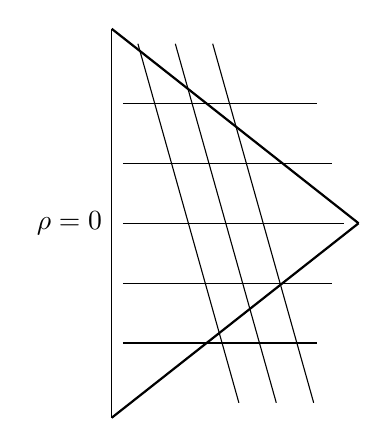
\begin{tikzpicture}[scale=0.95]
\draw (0,-2.6) -- (0,2.6);
\draw (0.15,1.6) -- (2.75,1.6);
\draw (0.15,0.8) -- (2.95,0.8);
\draw (0.15,0.0) -- (3.10,0.0);
\draw (0.15,-0.8) -- (2.95,-0.8);
\draw (0.15,-1.6) -- (2.75,-1.6);

\draw (0.35,2.40) -- (1.70,-2.40);
\draw (0.85,2.40) -- (2.20,-2.40);
\draw (1.35,2.40) -- (2.70,-2.40);

\draw[thick] (0,2.60) -- (3.30,0);
\draw[thick] (0,-2.60) -- (3.30,0);

\node[left] at (0,0) {\(\rho=0\)};
\end{tikzpicture}
\end{figure}

This is not yet the final Penrose diagram. It is the rule being enacted on the board: squash the infinite \(t\)-\(\rho\) grid into a finite region while preserving the \(45^\circ\) direction of radial light.

The more complete board result is then:

\begin{figure}[h]
\centering

\includegraphics[width=0.62\textwidth]{lecture_04_figure_06.png}
\end{figure}

A clean version of the compactified flat-space Penrose diagram is:

\begin{figure}[h]
\centering
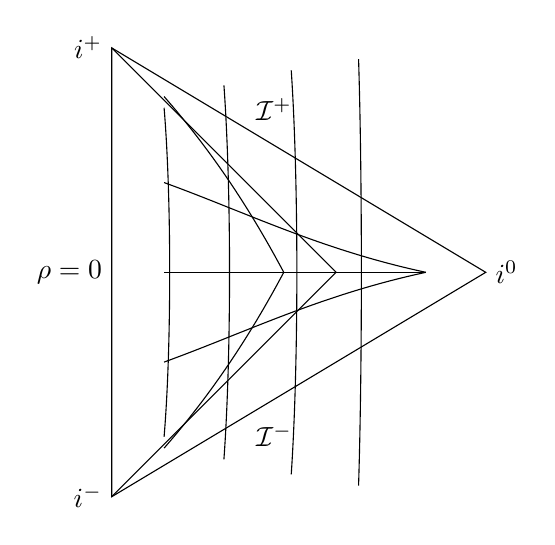
\begin{tikzpicture}[scale=0.95]
\draw (0,-3) -- (0,3) -- (5,0) -- cycle;

\draw (0.7,-2.35) .. controls (1.4,-1.55) and (1.9,-0.75) .. (2.3,0);
\draw (0.7,2.35) .. controls (1.4,1.55) and (1.9,0.75) .. (2.3,0);

\draw (0.7,-1.2) .. controls (1.8,-0.8) and (2.8,-0.3) .. (4.2,0);
\draw (0.7,0.0) .. controls (1.8,0.0) and (2.8,0.0) .. (4.2,0);
\draw (0.7,1.2) .. controls (1.8,0.8) and (2.8,0.3) .. (4.2,0);

\draw (0.7,-2.2) .. controls (0.8,-1.0) and (0.8,1.0) .. (0.7,2.2);
\draw (1.5,-2.5) .. controls (1.6,-1.1) and (1.6,1.1) .. (1.5,2.5);
\draw (2.4,-2.7) .. controls (2.5,-1.2) and (2.5,1.2) .. (2.4,2.7);
\draw (3.3,-2.85) .. controls (3.35,-1.25) and (3.35,1.25) .. (3.3,2.85);

\draw (0,-3) -- (3,0);
\draw (0,3) -- (3,0);

\node[left] at (0,3) {$i^+$};
\node[left] at (0,-3) {$i^-$};
\node[right] at (5,0) {$i^0$};
\node[above right] at (1.8,1.9) {$\mathcal{I}^+$};
\node[below right] at (1.8,-1.9) {$\mathcal{I}^-$};
\node[left] at (0,0) {$\rho=0$};
\end{tikzpicture}
\end{figure}

The notation here is the standard cleaned notation for Susskind's spoken labels:
\begin{equation}
i^+,\quad i^-,\quad i^0,\quad \mathcal{I}^+,\quad \mathcal{I}^-.
\end{equation}
The left boundary is the timelike axis \(\rho=0\). The right tip is spacelike infinity \(i^0\). The slanted upper and lower boundaries are future and past null infinity, the ``scri plus'' and ``scri minus'' of the lecture.

\begin{remark}
As Susskind later emphasizes in response to a question, the \(45^\circ\) rule is a rule for radial light rays. A light ray that misses the origin is not purely radial in the reduced two-dimensional description and need not be represented by a straight \(45^\circ\) line throughout.
\end{remark}

Only after flat space has been taught as a reading exercise does Susskind turn back to the black hole. The causal sketch from earlier in the lecture is the pre-compactification object to be ``squished.''

\begin{figure}[h]
\centering

\includegraphics[width=0.48\textwidth]{lecture_04_figure_04.png}
\end{figure}

A standard cautious reconstruction of the eternal Schwarzschild Penrose diagram is then:

\begin{figure}[h]
\centering
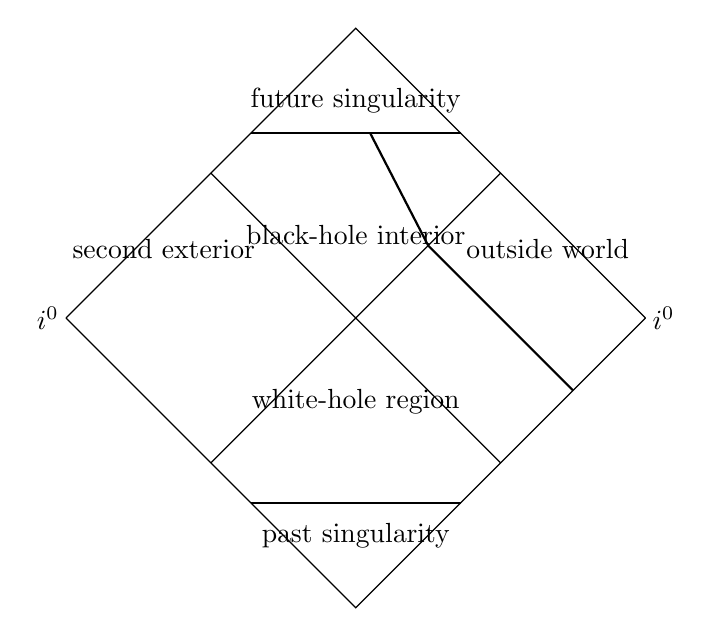
\begin{tikzpicture}[scale=0.92]
\coordinate (L) at (-4,0);
\coordinate (R) at (4,0);
\coordinate (UL) at (-2,2);
\coordinate (UR) at (2,2);
\coordinate (DL) at (-2,-2);
\coordinate (DR) at (2,-2);
\coordinate (T) at (0,4);
\coordinate (B) at (0,-4);
\coordinate (C) at (0,0);

\draw (L) -- (UL) -- (T) -- (UR) -- (R);
\draw (L) -- (DL) -- (B) -- (DR) -- (R);

\draw (UL) -- (C) -- (UR);
\draw (DL) -- (C) -- (DR);

\draw[thick] (-1.45,2.55) -- (1.45,2.55);
\draw[thick] (-1.45,-2.55) -- (1.45,-2.55);

\node at (0,3.0) {future singularity};
\node at (0,-3.0) {past singularity};
\node at (2.65,0.95) {outside world};
\node at (-2.65,0.95) {second exterior};
\node at (0,1.15) {black-hole interior};
\node at (0,-1.15) {white-hole region};
\node at (4.25,0) {$i^0$};
\node at (-4.25,0) {$i^0$};

\draw[thick] (3.0,-1.0) -- (1.0,1.0);
\draw[thick] (1.0,1.0) -- (0.2,2.55);
\end{tikzpicture}
\end{figure}

The diagram collects in one place much of what the lecture has already established locally. Radial null rays still move at \(45^\circ\). An inward-directed light ray from the exterior crosses the horizon and terminates on the future singularity. The upper triangular region is the black-hole interior. The lower one is the white-hole region. The right-hand diamond is the exterior world in which Bob lives. The left-hand diamond is a second asymptotic exterior region present in the eternal Schwarzschild solution.

Susskind's next move is to undercut the physical importance of half this picture. The second exterior and the white-hole half are artifacts of an eternal solution. They are not the geometry of an ordinary black hole formed in nature.

\section{Real Black Holes and the Birkhoff-Theorem Preview}

The lecture closes by shifting from eternal black holes to real ones. In nature, black holes are formed. Susskind imagines matter, even a cloud of photons, coming in from far away. Since photons carry energy and therefore gravitate, enough incoming radiation concentrated in a sufficiently small region can form a black hole. The question is then not what an eternal Schwarzschild solution looks like, but how one glues a nearly empty pre-collapse spacetime to a black-hole spacetime in the future.

To prepare that construction, Susskind introduces first the Newtonian theorem and then its general-relativistic analogue.

\begin{proposition}[Newton's shell theorem]
For a spherically symmetric shell of total mass \(M\), the Newtonian gravitational field vanishes in the interior of the shell, while in the exterior it is exactly the same as the field of a point mass \(M\) placed at the center.
\end{proposition}

Susskind phrases this in the language of lines of force or flow lines of a fluid. Inside the shell there is no place for the symmetric inward flow to go, so the field must vanish. Outside the shell the lines of force are exactly those of a point mass at the center. He also emphasizes that this remains true if the shell changes radius in time, provided the total mass is conserved.

The general-relativistic statement is Birkhoff's theorem in the operational form needed for the next lecture.

\begin{theorem}[Birkhoff's theorem in the form used in the lecture]
For a spherically symmetric shell of total mass \(M\), the spacetime inside the shell is flat Minkowski spacetime, while the spacetime outside the shell is the Schwarzschild geometry of mass \(M\).
\end{theorem}

The two pieces to be patched together are therefore
\begin{align}
ds^2_{\text{inside}} &= -dt^2+dx^2+dy^2+dz^2,\\
ds^2_{\text{outside}} &= \text{Schwarzschild}(M).
\end{align}
As the shell contracts, its radius changes but its total mass does not. The boundary between the flat interior and the Schwarzschild exterior moves with time. That moving interface is exactly the structure Susskind wants for the next lecture, where the eternal diagram will finally be replaced by the spacetime of an actually formed black hole.

\section{Summary}

The lecture begins by returning to the near-horizon geometry in the variables \(\rho\) and \(\omega\), so that the local black-hole metric can be written as
\[
ds^2=-\rho^2\,d\omega^2+d\rho^2.
\]
From there Susskind asks how this local form connects to the far region, and he answers that question first by a cleaned asymptotic comparison and then by the Euclidean cigar analogy. With that intuition in hand, he turns the metric into a causal story: horizons as one-way barriers, Bob outside, Alice falling in, redshift, fading signals, and the feet-first thought experiment.

Only after that long operational discussion does he introduce the singularity and the coordinate interchange across \(r=2MG\), and from there the lecture naturally reaches the time-reversed white-hole extension. The white hole is left mathematically possible but physically downgraded by entropy. After the break, Penrose diagrams compress the same causal content into finite pictures, first for flat spacetime and then for eternal Schwarzschild. The chapter ends where the lecture ends: eternal black holes are not the real story, and Birkhoff's theorem provides the bridge to the next lecture's construction of black-hole formation by collapse.